\documentclass{beamer}

% ── Theme: Metropolis ────────────────────────────────────────────────────────
\usetheme{metropolis}
\metroset{sectionpage=none, subsectionpage=none, progressbar=frametitle}

% ── Packages ─────────────────────────────────────────────────────────────────
\usepackage{amsmath, amssymb, listings, xcolor}
\usepackage{tikz}
\usetikzlibrary{positioning, arrows.meta, shapes}

% ── Global TikZ styles (unchanged from v3) ────────────────────────────────────
\tikzset{
  stage/.style={
    draw, rectangle,
    minimum width=1.40cm, minimum height=0.65cm,
    fill=blue!25, font=\small\bfseries, align=center
  },
  blk/.style={
    draw, rectangle,
    minimum width=0.60cm, minimum height=0.38cm,
    fill=blue!25, font=\tiny\bfseries,
    inner sep=0pt, align=center
  },
  stl/.style={
    draw, rectangle,
    minimum width=0.60cm, minimum height=0.38cm,
    fill=red!30, font=\tiny\bfseries,
    inner sep=0pt, align=center
  },
  emp/.style={minimum width=0.60cm, minimum height=0.38cm},
  harr/.style={-{Stealth}, thick},
  fwdarr/.style={-{Stealth}, thick, dashed, green!60!black},
}

% ── Title metadata ───────────────────────────────────────────────────────────
\title{Understanding Pipelining Hazards}
\subtitle{BLG 483E -- Artificial Intelligence}
\author{salihsefer36}
\institute{Istanbul Technical University \\[0.4em]
           \footnotesize\itshape Generated with AI assistance,
           refined over 4 iterations.}
\date{\today}

% ─────────────────────────────────────────────────────────────────────────────
\begin{document}
% ─────────────────────────────────────────────────────────────────────────────

% ══════════════════════════════════════════════════════════════════════════════
% Slide 1 — Title
% ══════════════════════════════════════════════════════════════════════════════
\begin{frame}
  \titlepage
\end{frame}

% ══════════════════════════════════════════════════════════════════════════════
% Slide 2 — Learning Objectives  [NEW]
% ══════════════════════════════════════════════════════════════════════════════
\begin{frame}{Learning Objectives}
  After this lecture, you will be able to:
  \begin{enumerate}
    \item \textbf{Identify} the three classes of pipeline hazards --- data,
          structural, and control --- and give a concrete real-world analogy
          for each.
    \item \textbf{Apply} forwarding and stall-insertion logic to a given
          instruction sequence, and calculate the resulting stall count and
          total cycle time.
    \item \textbf{Compare} hardware mitigation strategies (forwarding,
          branch prediction, compiler scheduling) and explain which is most
          effective for each hazard class.
  \end{enumerate}
\end{frame}

% ══════════════════════════════════════════════════════════════════════════════
% Slide 3 — Table of Contents  [NEW]
% ══════════════════════════════════════════════════════════════════════════════
\begin{frame}{Outline}
  \tableofcontents
\end{frame}

% ════════════════════════════════════════════════════════════════
\section{What is Pipelining?}
% ════════════════════════════════════════════════════════════════

% ══════════════════════════════════════════════════════════════════════════════
% Slide 4 — Introduction to CPU Pipelining  [v3 + Intuition block]
% ══════════════════════════════════════════════════════════════════════════════
\begin{frame}{Introduction to CPU Pipelining}
  \textit{Think of a restaurant: one waiter takes orders, one chef cooks,
  another plates, another serves. If one person did everything per customer,
  the restaurant would serve one table at a time. A CPU pipeline works
  exactly the same way.}

  \smallskip
  \begin{itemize}
    \item A pipeline splits every instruction into 5 stages that run
          \textbf{simultaneously} for different instructions:
          \textbf{IF} (fetch), \textbf{ID} (decode), \textbf{EX} (execute),
          \textbf{MEM} (memory), \textbf{WB} (write result).
    \item When the assembly line runs smoothly, the CPU completes roughly
          one instruction per clock cycle (instead of one every 5 cycles).
    \item A \textbf{hazard} is anything that breaks the smooth flow ---
          a conflict that forces a stage to wait or throw away work.
    \item Hazards come in three flavours: \textbf{data}, \textbf{structural},
          and \textbf{control}.
  \end{itemize}

  \begin{block}{Intuition}
    \small The pipeline's power is \emph{overlap}, not speed. A hazard
    matters only when it destroys that overlap --- each stall is a stage
    that sat idle.
  \end{block}
\end{frame}

% ══════════════════════════════════════════════════════════════════════════════
% Slide 5 — The 5-Stage Pipeline  [v3 — TikZ Diagram 1, unchanged]
% ══════════════════════════════════════════════════════════════════════════════
\begin{frame}{The 5-Stage Pipeline}
  \begin{center}
  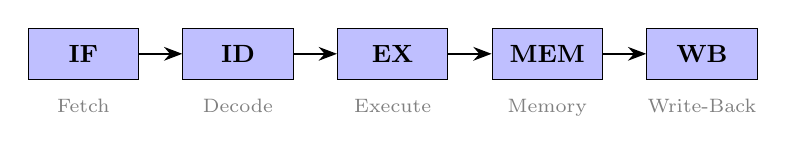
\begin{tikzpicture}
    \node[stage]                      (IF)  {IF};
    \node[stage, right=0.55cm of IF]  (ID)  {ID};
    \node[stage, right=0.55cm of ID]  (EX)  {EX};
    \node[stage, right=0.55cm of EX]  (MEM) {MEM};
    \node[stage, right=0.55cm of MEM] (WB)  {WB};
    \draw[harr] (IF)--(ID);
    \draw[harr] (ID)--(EX);
    \draw[harr] (EX)--(MEM);
    \draw[harr] (MEM)--(WB);
    \node[below=0.12cm of IF,  font=\scriptsize, text=gray] {Fetch};
    \node[below=0.12cm of ID,  font=\scriptsize, text=gray] {Decode};
    \node[below=0.12cm of EX,  font=\scriptsize, text=gray] {Execute};
    \node[below=0.12cm of MEM, font=\scriptsize, text=gray] {Memory};
    \node[below=0.12cm of WB,  font=\scriptsize, text=gray] {Write-Back};
  \end{tikzpicture}
  \end{center}

  \smallskip
  \begin{itemize}
    \item \textbf{IF} fetches the raw binary instruction from the instruction cache.
    \item \textbf{ID} decodes opcodes and reads source-register values.
    \item \textbf{EX} runs the ALU operation (add, subtract, address compute).
    \item \textbf{MEM} reads from or writes to the data cache.
    \item \textbf{WB} commits the computed value to the destination register.
  \end{itemize}
  \begin{center}
    \scriptsize In a \emph{hazard-free} pipeline a new instruction enters
    IF every cycle. \textbf{Hazards break this ideal.}
  \end{center}
\end{frame}

% ════════════════════════════════════════════════════════════════
\section{Data Hazards}
% ════════════════════════════════════════════════════════════════

% ══════════════════════════════════════════════════════════════════════════════
% Slide 6 — Data Hazards: Types  [v3 + Intuition block]
% ══════════════════════════════════════════════════════════════════════════════
\begin{frame}{Data Hazards --- Types}
  \textit{Imagine a relay race where runner B must grab the baton from runner A
  before sprinting. If B takes off before A arrives, the handoff fails.
  Data hazards are exactly that: one instruction needs a value the previous
  one has not finished computing yet.}

  \smallskip
  \begin{itemize}
    \item \textbf{RAW} (Read-After-Write, ``true dependence''): the most common
          type. Instruction B tries to read a register before instruction A has
          written its result. \textit{Runner B sprints before the baton arrives.}
    \item \textbf{WAR} (Write-After-Read, ``anti-dependence''): B overwrites a
          register that A is still reading. \textit{Chef B cleans the pan chef A
          is still using.}
    \item \textbf{WAW} (Write-After-Write, ``output dependence''): two
          instructions write the same register; the second write must dominate.
          \textit{Two workers file the same report --- only the later one counts.}
  \end{itemize}

  \begin{block}{Intuition}
    \small RAW is the only \emph{true} dependence. WAR and WAW are structural
    artefacts --- they vanish in processors that use register renaming.
  \end{block}
\end{frame}

% ══════════════════════════════════════════════════════════════════════════════
% Slide 7 — Data Hazards: Detection & Mitigation  [v3 + Intuition block]
% ══════════════════════════════════════════════════════════════════════════════
\begin{frame}{Data Hazards --- Detection \& Mitigation}
  \textit{Think of a traffic officer watching an intersection. When two cars
  are about to collide, the officer either holds one back (stall) or waves it
  through a special shortcut lane (forwarding).}

  \smallskip
  \begin{itemize}
    \item \textbf{Detection:} A hazard detection unit checks the pipeline
          registers (ID/EX, EX/MEM, MEM/WB) every cycle to spot conflicts
          before they corrupt results.
    \item \textbf{Stall (interlock):} Freeze the fetch and decode stages and
          insert a bubble (a ``do nothing'' slot) --- like a one-cycle red light.
    \item \textbf{Forwarding (bypassing):} Route the result directly from one
          stage to the next instruction's input, skipping the register file.
          Eliminates most RAW stalls completely.
    \item \textbf{Load-use exception:} A load followed immediately by a
          dependent instruction cannot be saved by forwarding --- one stall is
          unavoidable.
  \end{itemize}

  \begin{block}{Intuition}
    \small Forwarding trades extra wires for time. The load-use case is the one
    penalty no wiring can eliminate: you \emph{must} wait for the memory read.
  \end{block}
\end{frame}

% ══════════════════════════════════════════════════════════════════════════════
% Slide 8 — Worked Example: RAW Hazard & Forwarding  [v3 — TikZ #2 + tabular]
% ══════════════════════════════════════════════════════════════════════════════
\begin{frame}{Worked Example: RAW Hazard \& Forwarding}
  \texttt{\scriptsize I1:~ADD~R1,R2,R3} \qquad
  \texttt{\scriptsize I2:~SUB~R4,\textcolor{red}{R1},R5}
  \;{\scriptsize --- I2 reads R1 produced by I1 (\textbf{RAW} dependence)}

  \smallskip
  \begin{columns}[T]
    \begin{column}{0.50\textwidth}
      \centering{\small\textbf{Without Forwarding}}
      \begin{center}
      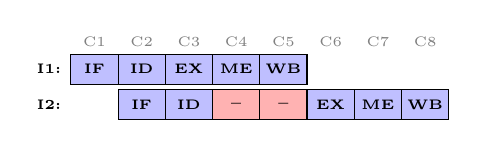
\begin{tikzpicture}
        \foreach \idx/\cx in
          {1/0.30, 2/0.90, 3/1.50, 4/2.10, 5/2.70, 6/3.30, 7/3.90, 8/4.50}{
          \node[font=\tiny, text=gray] at (\cx, 0.80) {C\idx};
        }
        \node[font=\tiny\bfseries, anchor=east] at (0.00, 0.45) {I1:};
        \node[blk] at (0.30, 0.45) {IF};
        \node[blk] at (0.90, 0.45) {ID};
        \node[blk] at (1.50, 0.45) {EX};
        \node[blk] at (2.10, 0.45) {ME};
        \node[blk] at (2.70, 0.45) {WB};
        \node[emp] at (3.30, 0.45) {};
        \node[emp] at (3.90, 0.45) {};
        \node[emp] at (4.50, 0.45) {};
        \node[font=\tiny\bfseries, anchor=east] at (0.00, 0.00) {I2:};
        \node[emp] at (0.30, 0.00) {};
        \node[blk] at (0.90, 0.00) {IF};
        \node[blk] at (1.50, 0.00) {ID};
        \node[stl] at (2.10, 0.00) {--};
        \node[stl] at (2.70, 0.00) {--};
        \node[blk] at (3.30, 0.00) {EX};
        \node[blk] at (3.90, 0.00) {ME};
        \node[blk] at (4.50, 0.00) {WB};
      \end{tikzpicture}
      \end{center}
      \centering{\scriptsize \textcolor{red}{2 stall cycles} $\Rightarrow$ \textbf{8 cycles}}
    \end{column}
    \begin{column}{0.50\textwidth}
      \centering{\small\textbf{With Forwarding}}
      \begin{center}
      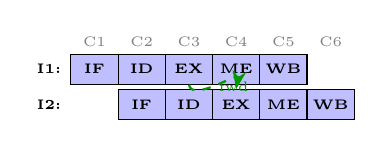
\begin{tikzpicture}
        \foreach \idx/\cx in
          {1/0.30, 2/0.90, 3/1.50, 4/2.10, 5/2.70, 6/3.30}{
          \node[font=\tiny, text=gray] at (\cx, 0.80) {C\idx};
        }
        \node[font=\tiny\bfseries, anchor=east] at (0.00, 0.45) {I1:};
        \node[blk]        at (0.30, 0.45) {IF};
        \node[blk]        at (0.90, 0.45) {ID};
        \node[blk] (i1ex) at (1.50, 0.45) {EX};
        \node[blk]        at (2.10, 0.45) {ME};
        \node[blk]        at (2.70, 0.45) {WB};
        \node[emp]        at (3.30, 0.45) {};
        \node[font=\tiny\bfseries, anchor=east] at (0.00, 0.00) {I2:};
        \node[emp]        at (0.30, 0.00) {};
        \node[blk]        at (0.90, 0.00) {IF};
        \node[blk]        at (1.50, 0.00) {ID};
        \node[blk] (i2ex) at (2.10, 0.00) {EX};
        \node[blk]        at (2.70, 0.00) {ME};
        \node[blk]        at (3.30, 0.00) {WB};
        \draw[fwdarr] (i1ex.south)
          to[out=-80, in=80]
          node[right, font=\tiny, green!60!black, inner sep=1pt] {fwd}
          (i2ex.north);
      \end{tikzpicture}
      \end{center}
      \centering{\scriptsize \textcolor{green!60!black}{0 stalls} $\Rightarrow$ \textbf{6 cycles}}
    \end{column}
  \end{columns}

  \smallskip
  {\scriptsize\textbf{Step-by-step (no fwd vs.\ fwd):}}
  \begin{center}
  {\scriptsize\setlength{\tabcolsep}{3.5pt}
  \begin{tabular}{l|cccccccc}
    \hline
    Instruction & C1 & C2 & C3 & C4 & C5 & C6 & C7 & C8 \\
    \hline
    I1 (ADD R1,R2,R3)   & IF & ID & EX & ME & WB &    &    &    \\
    I2 without fwd      &    & IF & ID & \textcolor{red}{--} & \textcolor{red}{--} & EX & ME & WB \\
    I2 with fwd         &    & IF & ID & EX & ME & WB &    &    \\
    \hline
  \end{tabular}}
  \end{center}
  {\scriptsize\textbf{Result:} No fwd: \textbf{2 stalls} (8 cycles). Fwd: \textbf{0 stalls}
  (6 cycles) --- \textbf{25\% speedup}.}
\end{frame}

% ════════════════════════════════════════════════════════════════
\section{Structural \& Control Hazards}
% ════════════════════════════════════════════════════════════════

% ══════════════════════════════════════════════════════════════════════════════
% Slide 9 — Structural Hazards  [v3 + Intuition block]
% ══════════════════════════════════════════════════════════════════════════════
\begin{frame}{Structural Hazards}
  \textit{Two delivery trucks arriving at a warehouse with a single loading dock
  at the same time: one must wait. Structural hazards are the same idea ---
  two pipeline stages need the same piece of hardware simultaneously.}

  \smallskip
  \begin{itemize}
    \item \textbf{Memory conflict:} Without separate instruction and data caches,
          the Fetch and Memory stages cannot both run in the same cycle.
    \item \textbf{Register write-port conflict:} A single-port register file
          cannot accept two write-back results simultaneously.
          \textit{One printer, two jobs queued at once.}
    \item \textbf{Multi-cycle unit contention:} Slow FP operations (divide,
          square root) tie up a shared unit for many cycles.
    \item \textbf{Fixes:} Duplicate hardware, time-share the resource, or
          let the compiler insert independent work between the conflicting
          instructions.
  \end{itemize}

  \begin{block}{Intuition}
    \small Every structural hazard has one root cause: more demand than supply
    for a hardware resource. The fix is always either \emph{add supply} or
    \emph{stagger demand}.
  \end{block}
\end{frame}

% ══════════════════════════════════════════════════════════════════════════════
% Slide 10 — Control Hazards  [v3 + Intuition block]
% ══════════════════════════════════════════════════════════════════════════════
\begin{frame}{Control Hazards}
  \textit{You are driving and your GPS says ``turn left'' --- but you are
  already in the right lane three blocks back. A branch hazard is the same:
  the CPU grabs the wrong next instructions before it knows which way a
  branch goes.}

  \smallskip
  \begin{itemize}
    \item Branch outcome is resolved at EX, so 2 instructions are already
          fetched for the wrong path and must be \textbf{flushed}, wasting
          2 cycles.
    \item \textbf{Static prediction:} Always guess ``not taken''. Simple,
          but wrong for loops.
    \item \textbf{Dynamic prediction (2-bit counter):} Learns from past
          behaviour --- like a GPS that remembers your usual route.
    \item \textbf{Branch Target Buffer (BTB):} Caches the destination address
          so the CPU can jump immediately.
    \item \textbf{Delayed branch:} The compiler fills the post-branch slot
          with a useful instruction, recovering one cycle for free.
  \end{itemize}

  \begin{block}{Intuition}
    \small Branch prediction is a bet. A good predictor wins $>$95\% of the
    time in real programs. The cost of losing scales with pipeline depth.
  \end{block}
\end{frame}

% ════════════════════════════════════════════════════════════════
\section{Mitigation Techniques}
% ════════════════════════════════════════════════════════════════

% ══════════════════════════════════════════════════════════════════════════════
% Slide 11 — Hazard Mitigation Summary  [v3 + Intuition block]
% ══════════════════════════════════════════════════════════════════════════════
\begin{frame}{Hazard Mitigation Summary}
  \textit{A factory supervisor has three tools: a stop button (stall), a
  conveyor shortcut (forwarding), and a smart pre-planned schedule (compiler
  reordering). Together they keep the assembly line moving.}

  \smallskip
  \begin{itemize}
    \item \textbf{Stall:} Freeze the front of the pipeline and insert a bubble
          --- buys time, but costs cycles.
    \item \textbf{Forwarding:} A hardware shortcut routing a result directly to
          the next instruction's input --- cuts most RAW stalls to zero.
    \item \textbf{Load-use stall:} Forwarding cannot rescue this case; one
          wasted cycle is unavoidable.
    \item \textbf{Branch delay slot:} Filling the post-branch slot with real
          work (not \texttt{NOP}) recovers a cycle for free.
    \item \textbf{Compiler scheduling:} Static reordering eliminates many
          hazards before the hardware ever encounters them.
  \end{itemize}

  \begin{block}{Intuition}
    \small Hardware patches runtime hazards; the compiler eliminates
    compile-time ones. Out-of-order CPUs blur this boundary by doing both
    dynamically.
  \end{block}
\end{frame}

% ════════════════════════════════════════════════════════════════
\section{Summary}
% ════════════════════════════════════════════════════════════════

% ══════════════════════════════════════════════════════════════════════════════
% Slide 12 — References  [v3 — unchanged]
% ══════════════════════════════════════════════════════════════════════════════
\begin{frame}{References}
  \begin{thebibliography}{9}
    \bibitem{patterson} Patterson, D.\,A. and Hennessy, J.\,L.
      \textit{Computer Organization and Design: The Hardware/Software Interface},
      5th ed. Morgan Kaufmann, 2014.
    \bibitem{hennessy} Hennessy, J.\,L. and Patterson, D.\,A.
      \textit{Computer Architecture: A Quantitative Approach},
      6th ed. Morgan Kaufmann, 2017.
  \end{thebibliography}
\end{frame}

% ══════════════════════════════════════════════════════════════════════════════
% Slide 13 — Real-World Context  [NEW — second-to-last]
% ══════════════════════════════════════════════════════════════════════════════
\begin{frame}{Real-World Context}
  \textit{Pipelining hazards are not textbook abstractions --- they determine
  the performance of every processor you interact with daily.}

  \medskip
  \begin{itemize}
    \item \textbf{Modern x86 (Intel/AMD Core series):} 14--20+ pipeline stages;
          out-of-order execution and Tomasulo's algorithm handle RAW hazards
          dynamically via register renaming, eliminating most stalls at runtime.
          Branch predictors achieve $>$98\% accuracy on typical workloads.
    \item \textbf{ARM Cortex family:} Cortex-A53 is a simple in-order pipeline
          where hazard avoidance is critical. Cortex-A76 is fully out-of-order
          with speculative execution --- the same hazard concepts, radically
          different hardware solutions.
    \item \textbf{GPU SIMT / CUDA streams:} GPUs hide pipeline latency not
          with forwarding but with \emph{warp switching} --- when one warp
          stalls on memory, another runs instantly. Thousands of threads mask
          penalties that would cripple a CPU pipeline.
  \end{itemize}
\end{frame}

% ══════════════════════════════════════════════════════════════════════════════
% Slide 14 — Summary & Common Pitfalls  [NEW — final]
% ══════════════════════════════════════════════════════════════════════════════
\begin{frame}{Summary \& Common Pitfalls}
  \textbf{Key takeaways:}
  \begin{itemize}
    \item \textbf{Three hazard classes:} data (RAW / WAR / WAW), structural
          (resource conflict), control (branch uncertainty).
    \item \textbf{Forwarding} eliminates most RAW stalls; the
          \textbf{load-use} case always costs exactly 1 cycle --- no exception.
    \item \textbf{Dynamic branch prediction} (2-bit counter + BTB) cuts
          control-hazard penalties to near-zero for predictable code.
  \end{itemize}

  \smallskip
  \textbf{Common misconceptions:}
  \begin{itemize}
    \item \textit{``Forwarding solves all data hazards.''} --- False: a load
          followed by an immediately dependent instruction always stalls once.
    \item \textit{``Deeper pipelines are always faster.''} --- False: deeper
          pipelines amplify branch penalties (e.g., Intel Pentium 4 Prescott,
          31 stages, notorious for branch-miss performance).
  \end{itemize}

  \begin{alertblock}{Test Yourself}
    \small \texttt{I1: LW~R1,0(R2)} \enspace \texttt{I2: ADD~R3,R1,R4}
    \enspace \texttt{I3: SUB~R5,R3,R6} \\
    With full forwarding enabled, how many total stall cycles does this
    3-instruction sequence require, and which instruction pair causes the stall?
  \end{alertblock}
\end{frame}

\end{document}
